\section{\ours Methodology}
~\ours relies on a parallel-tracking-and-mapping architecture, as first defined by Klein and Murray~\cite{klein2007parallel} and adopted by most visual SLAM implementations~\cite{campos2021orb}. \cref{fig:ovo} shows an overview of \ours.
It takes as input a stream of RGB-D keyframes ($\{ k_0, \hdots, k_n\}$ in the figure) and their respective poses and local point clouds. 
%Keyframe-based SLAM pipelines are common in the literature and \ours can be integrated with them, as we will show in the experimental results. 
From this 3D representation, \cref{sec:map}, \ours extracts and tracks a set of 3D segments covering the whole representation (\emph{3D segment mapper} in the figure, detailed in~\cref{sec:mapper}). 
We compute a CLIP descriptor per each segment's viewpoint merging 3 different CLIPs (\emph{CLIP merging} in the figure, detailed in~\cref{sec:merging}). Then assign to the 3D segment the most representative descriptor, \cref{sec:sem_computation}. 
When the SLAM module performs a loop closure or bundle-adjustment optimization, a routine searches for repeated 3D segments, and fuses those that were not correctly tracked,~\cref{sec:loop_closure}.
%------------------------------------------------------------------------------
\subsection{Map Definition}
\label{sec:map}
%------------------------------------------------------------------------------
%
%\ours assumes a parallel-tracking-and-mapping architecture, as first defined by Klein and Murray~\cite{klein2007parallel} and adopted by most visual SLAM implementations~\cite{campos2021orb}.
Its input is an RGB-D video \(\mathcal{V} = \{f_0, \hdots, f_\tau\}\), \(f_\tau \in \mathbb{N}_{\leq 255}^{w \times h \times 3} \times \mathbb{R}_{>0}\) representing the RGB-D frame of size $w \times h$ captured at time step \(\tau\). A SLAM front-end estimates in real-time the pose \(T_n\) of every frame \(f_\tau\) in the world reference frame. The SLAM back-end selects a set of keyframes \(\mathcal{K} = \{k_0, \hdots\, k_n\} \subset \mathcal{V}\) from which it iteratively refines their poses $\mathcal{T} = \{T_{0}, \hdots, T_{n}\}$, \(T_{n} \in SE(3)\) asynchronously, at a rate lower than the video rate of the tracking thread. 

Our scene representation or `map' $\mathcal{M} = \{ \mathcal{T}, \mathcal{P}, \mathcal{S} \}$, consists on these keyframe poses $\mathcal{T}$, a point cloud $\mathcal{P} = \{P_0, \hdots, P_m\}$ and a set of 3D segments $\mathcal{S} = \{S_0, \hdots, S_q\}$, being $q$ the identifier of the last added segment. 
Every map point $P = \big( \begin{bmatrix}
x & y & z
\end{bmatrix}^\top, \ l_p \big)$ is defined by its 3D coordinates $\begin{bmatrix}
x & y & z 
\end{bmatrix}^\top \in \mathbb{R}^3$ and a discrete label $l_p \in \{-1, 0, 1, \hdots, q\}$, $l_p>-1$ indicating the 3D segment the point belongs to, and $l_p=-1$ indicating that it is unassigned. 
The dense point cloud \(\mathcal{P}\) is built concatenating at each keyframe \(k_n\) the estimated 3D points \(\mathcal{P}_n\) provided by the SLAM front-end. 
If the SLAM front-end does not estimate a dense point cloud, \(\mathcal{P}_n\) is computed as the unprojection of the input depth map to 3D using the estimated camera pose \(T_{n} \in SE(3)\). To avoid \(\mathcal{P}\) growing unconstrained, a pixel is not projected to 3D if a previously unoccluded 3D point falls inside its neighborhood when projected back to 2D. 
For every 3D point, occlusion is assessed by comparing its projected depth to its measured depth in the 2D pixel it is projected.
Every 3D segment $S = \left( \mathbf{d}, \kappa \right)$ has a unique identifier, its semantics are described by a CLIP feature $\mathbf{d} \in \mathbb{R}^d$, and stores in a heap $\kappa$ the indices of the best keyframes in which $S$ was seen, ordered by visibility scores.
%------------------------------------------------------------------------------
\subsection{3D Segment Mapper}
\label{sec:mapper}
%------------------------------------------------------------------------------
\begin{algorithm}[t]
\normalsize 
\caption{3D Segment Mapper} 
\begin{algorithmic}[1] 
%\normalsize
\footnotesize
\Function{3D\_segment\_mapper}{$\mathcal{P}$, $\mathcal{S}$, $k_n, T_n$}

    \State $\tilde{\mathcal{S}}_n\leftarrow$ segment\_keyframe$(k_n)$
    \State $\tilde{\mathcal{P}}_n \leftarrow$ project\_point\_cloud$(\mathcal{P},T_n)$
    \For{$\left(s, l_s\right) $ in $\tilde{\mathcal{S}}_n$} \Comment{For every 2D segment in $k_n$}
    \State $mode, v \leftarrow$ get\_label\_mode\_and\_votes$(\tilde{\mathcal{P}}_n,s,\epsilon)$
    \If{$v > \epsilon$} \Comment{\#votes greater than threshold}
    \If{$mode = -1$}
    \State $S_{q+1} \leftarrow$ new\_3D\_segment$(q+1, n, s)$
    \State $\mathcal{S} \leftarrow \mathcal{S} \cup\{S_{q+1}\}$
    \State $l_s \leftarrow q+1$
    \Else
    \State $\mathcal{S} \leftarrow$ update\_3D\_segment$(S_{mode}, n, s)$
    \State $l_s \leftarrow z_l$
    \EndIf
    \EndIf
    \EndFor
    \State $\tilde{\mathcal{S}}_n \leftarrow$ merge\_and\_prune\_2D\_segments$(\tilde{\mathcal{S}}_n)$
    \State $\mathcal{P} \leftarrow$ update\_pcd\_labels$(\mathcal{P},\tilde{\mathcal{P}}_n, \tilde{\mathcal{S}}_n)$
    \State \Return $\mathcal{P}$, $\mathcal{S}, \tilde{\mathcal{S}}_n$
\EndFunction
\end{algorithmic}
\label{alg:3dsegmentor}
\end{algorithm}
\begin{figure*}[tb]
    \centering
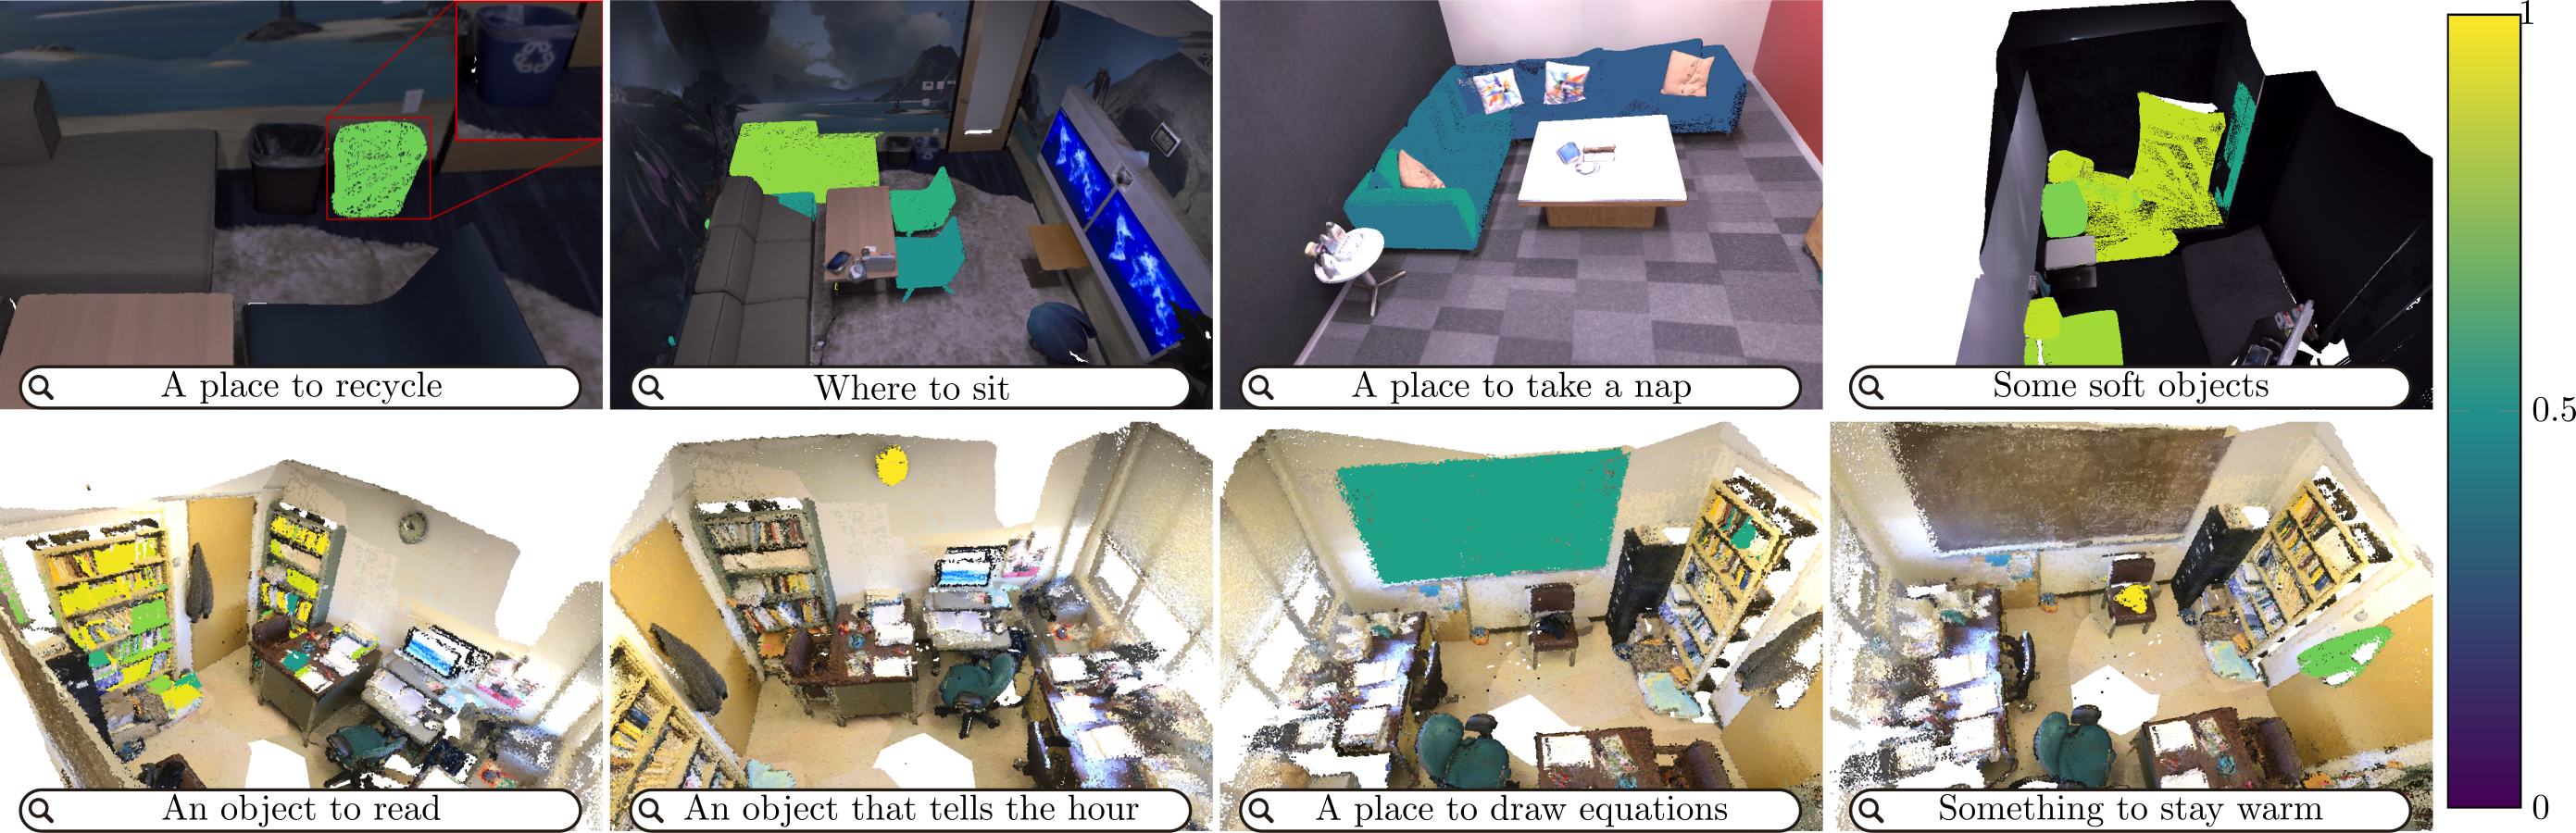
\includegraphics[width=\linewidth]{figures/images/gen_queries.png}
    \caption{\textbf{Out-of-distribution queries.} From left to right, top to bottom, observe how common-language queries allow to differentiate bins based on a recycling symbol; recongize sofas and chairs as places to sit; that you can take a nap in a sofa, pillows and couches are soft objects, and books are readable, that the clock tells the hour, the blackboard is to draw equations, and the jacket is something to stay warm. Colorbar shows similarity strength. 
    }
    \label{fig:gen_queries}    
\end{figure*}
For every new keyframe $k_n$, we run an image segmentation model that returns a set of 2D segments $\tilde{\mathcal{S}_n}=\{ \left(s_0,l_{s0}\right), \left(s_1,l_{s1}\right), \hdots\}$, each segment being composed of a mask $s$ and a label $l_s$, which is initialized as $l_s:=-1$. 
We then select the 3D map points in $k_n$'s frustum, project them to $k_n$, and remove occluded points by comparing their projected depth to the input depth. 
In this manner, we obtain the 2D point set $\tilde{\mathcal{P}}_n=\{p_0, p_1, \hdots\}$, for which $p = \big( \begin{bmatrix}
u & v
\end{bmatrix}^\top, \ l_p \big)$.
We compute the label mode of all points $p$ within a segment $s$, that we will represent slightly abusing notation as $z_l := \arg\max_{l_p}\left(\tilde{\mathcal{P}}\cap s\right)$. 
If the mode receives less votes \(v\) than a predefined threshold $\epsilon$, we discard $s$.
If not, two possibilities can occur:
\begin{enumerate}
    \item If $z_l\!=\!-1$, we set $z_l\!:=\!q\!+\!1$ and initialize a new 3D segment $S_{q+1}$ with an empty CLIP feature $\mathbf{d}$ (filled later as described in Sec.~\ref{sec:sem_computation}), and a keyframe heap $\kappa\!:=\!\{\left(n, r\right)\}$, initialized with $k_n$'s index and $s$' visibility score $r$.
    %
    \item Otherwise, 2D segment $s$ is a match for 3D segment $S_{z_l}$ and the keyframe will be inserted into \(\kappa\), and stored if it is one of the best views or if \(\kappa\) is not full.
\end{enumerate}
%
For both, the unassigned 3D points and 2D segment's labels, $l_p$ and  $l_s$ are updated to the identifier of the matched ${S}_{z_l}$.

After matching all 2D masks, those that share the same $l_s$ are merged.
Finally, once all masks are gathered in $\tilde{\mathcal{S}}_n$, the tuple $\big(k_n,\tilde{\mathcal{S}}_n\big)$ is pushed to the queue \(\mathcal{Q}\).
Keyframes and masks remain in $\mathcal{Q}$ until processing resources become available to compute the CLIP descriptors for the highest-scoring 2D segments. 
%
%
%------------------------------------------------------------------------------
\subsection{Loop Closure}
\label{sec:loop_closure}
%------------------------------------------------------------------------------
%
When the SLAM module closes a loop or completes a Global Bundle Adjustment, \ours updates both its map and the set of 3D instances. We denote both after the update as \(\mathcal{M}^\prime\) and \(\mathcal{S}^\prime\).
For each updated keyframe \(T_n^\prime\in\mathcal{T}^\prime\), its associated local point cloud is also updated by propagating the pose correction as \(
    \mathcal{P}_{n} := T_{n}^\prime \ T_{n}^{-1} \ \mathcal{P}_n
\). 
This transforms the points from the world frame to the original keyframe's and back using the updated pose \(T_{n}^\prime\).
Keyframes that are removed during SLAM optimization are discarded along with their associated 3D points.
After updating the 3D points, the temporary queue \(\mathcal{Q}\) is cleared. Next, the set of 3D instances \(\mathcal{S}^\prime\) is pruned by removing instances whose associated points were entirely deleted during optimization.
Following, instance fusion is performed by comparing remaining pairs of 3D instances. Two instances are merged if they satisfy the following criteria: \textbf{(1)} The distance between their point cloud centroids is \(<150\)cm, \textbf{(2)} the cosine similarity between their CLIPs is \(>0.8\), and \textbf{(3)} more than \(50\%\) of their points lie within $10$cm of a point in the other instance.
For a pair of segments \(S_i\) and \(S_j\) to be merged, their point indices are unified as \( \kappa_i := \kappa_i \cup \kappa_j \), and all map points previously labeled as \(j\) are reassigned to \(i\), i.e., 
\(\forall P_k \in \mathcal{P} | l_k = j ,\implies l_k := i\).
%
%------------------------------------------------------------------------------
\subsection{CLIP Descriptors
} \label{sec:sem_computation}
%------------------------------------------------------------------------------
%
When a tuple $\big(k_q,\tilde{\mathcal{S}}_q\big)$ is popped from $\mathcal{Q}$, only the matched 2D segments for which $k_q$ is still in the $\kappa$ of their 3D instance $S$ are selected. 
A CLIP descriptor $\mathbf{d}$ is computed for each of them as explained in \cref{sec:merging}. 
Then, the final descriptor for a 3D segment $S$ is selected between the 2D segments in its keyframes' heap $\kappa$, as the CLIP descriptor with the smallest aggregated distance to the rest.
To query the 3D semantic representation, text queries are encoded to CLIP space.
 Then, we compute the cosine similarity between the CLIP descriptor of the query and the descriptor $\mathbf{d}$ of each 3D segment in $\mathcal{S}$. 
%
\begin{figure*}[tb]
\centering
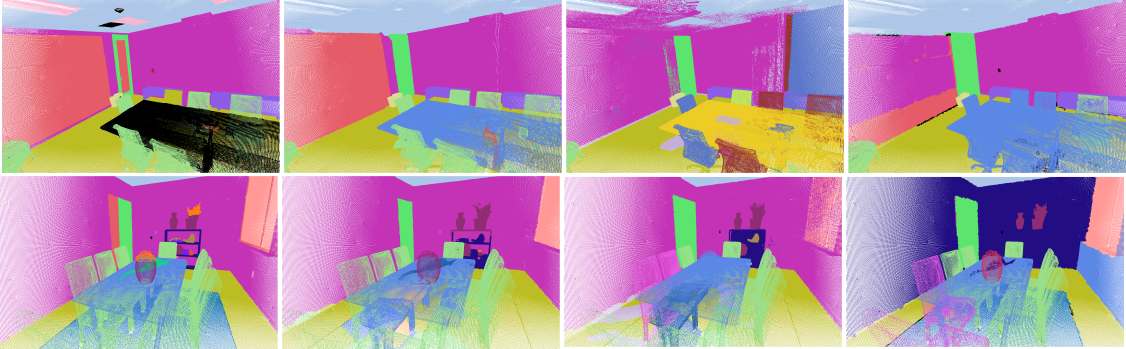
\includegraphics[width=\textwidth]{figures/images/replica.png}
\resizebox{\textwidth}{!}
{
\begin{tabular}{cccc}
        \vspace{-10px}\\
        \textit{\small \color{black} Ground truth} &
        \textit{\small \color{black} \ours -Gaussian-SLAM (ours)} &
        \textit{\small \color{black} HOV-SG~\cite{hovsg}} &
        \textit{\small \color{black} Open3DIS~\cite{nguyen2024open3dis}}\\
        \hspace{0.22\textwidth} &
        \hspace{0.22\textwidth} &
        \hspace{0.22\textwidth} &
        \hspace{0.22\textwidth}
    \end{tabular}
}
\resizebox{\textwidth}{!}{
\begin{tabular}{c}
\vspace{-22px}
\ColorMapCircle{r_panel}\,panel
\ColorMapCircle{r_vase}\,vase
\ColorMapCircle{r_clock}\,clock
\ColorMapCircle{r_pot}\,pot 
\ColorMapCircle{r_window}\,window
\ColorMapCircle{r_bottle}\,bottle
\ColorMapCircle{r_indoor-plant}\,indoor-plant
\ColorMapCircle{r_blinds}\,blinds
\ColorMapCircle{r_lamp}\,lamp
\ColorMapCircle{r_wall-plug}\,wall-plug
\small\ColorMapCircle{r_wall}\,wall
\ColorMapCircle{r_switch}\,switch
\ColorMapCircle{r_bench}\,bench\\ \vspace{14px}
\small\ColorMapCircle{r_box}\,box 
\ColorMapCircle{r_shelf}\,shelf
\ColorMapCircle{r_stool}\,stool
\ColorMapCircle{r_rug}\,rug
\ColorMapCircle{r_table}\,table
\ColorMapCircle{r_ceiling}\,ceiling
\ColorMapCircle{r_bowl}\,bowl
\ColorMapCircle{r_camera}\,camera
\ColorMapCircle{r_door}\,door
\ColorMapCircle{r_plate}\,plate
\ColorMapCircle{r_chair}\,chair
\ColorMapCircle{r_vent}\,vent
\ColorMapCircle{r_bin}\,bin
\ColorMapCircle{r_desk}\,desk
\ColorMapCircle{r_floor}\,floor
\ColorMapCircle{r_sculpture}\,sculpture
\end{tabular}
}
\vspace{-14px}
\caption{\textbf{3D semantic segmentation on Replica.} \ours yields more accurate results in comparison to the two best offline baselines.}

\label{fig:replica}
\end{figure*}



%\input{figures/fig_scannetv2}
%------------------------------------------------------------------------------
\subsection{CLIP Merging}
\label{sec:merging}
%------------------------------------------------------------------------------
Similarly to HOV-SG~\cite{hovsg}, for each 2D segment we compute three CLIP descriptors: 1) $\mathbf{d}_0$ for the full keyframe, 2) $\mathbf{d}_1$ for the segment masking the rest of the image out, and 3) $\mathbf{d}_2$ for the minimum bounding box that contains the segment.
In contrast, in our case, the CLIP descriptor $\mathbf{d}= \sum_{i=0}^2 \mathbf{w}_i \odot \mathbf{d}_i$ of a 2D segment is the result of merging the three descriptors $\mathbf{d}_{i=\{0, 1, 2\}}$ using a per-dimension weighted average with weights $\mathbf{w}_i \in \mathbb{R}^d$ ($\odot$ is the Hadamard product). Our weights $\mathbf{w}_{i=\{0, 1, 2\}}$ are predicted by a neural model, as shown in \cref{fig:ovo}. Note that HOV-SG's merging is done with hand-crafted scalar weights (\emph{i.e.}, $\mathbf{d}= \sum_{i=0}^2 {w}_i \mathbf{d}_i$, ${w}_i \in \mathbb{R}$).%, more details in \cref{sec:supp_CLIP_merging}.

As seen in 
\cref{fig:ovo}, the input to our CLIP merging  is three CLIPs $\mathbf{d}_{i=\{0, 1, 2\}}$. 
These are first passed by a transformer encoder, and the output is flattened and fed to a MLP, predicting the weights, and a softmax, forcing $\sum_{i=0}^2 \mathbf{w}_{i}=\mathbf{1}^d$.
Our \clipours is pre-trained following  SigLIP~\cite{zhai2023siglip}.
For a mini-batch \(\mathcal{B} = \left\{ (s_0, c_0), (s_1, c_1), \dots \right\}\) composed by pairs of 2D segments $s_j$ and semantic classes $c_j$, we minimize the sigmoid cosine similarity loss
%
\begin{equation}
   L = -\frac{1}{|\mathcal{B}|} \sum_{i=1}^{|\mathcal{B}|} \sum_{j=1}^{|\mathcal{B}|} \log\! \left( \frac{1}{1 \! +\! \exp(z_{ij}(-t \mathbf{d}_i \cdot \mathbf{y}_j + b))} \right)
\end{equation} 
%
between the merged CLIP descriptor \(\mathbf{d}_i\), and the CLIP embedding \(\mathbf{y}_j\) of the semantic class $c_j$ associated to the 2D segment $s_j$ in the same batch $\mathcal{B}$. \(z_{ij}\) is the label for a given image and class input, which equals \(1\) if they are paired and \(-1\) otherwise. \(b\) and \(t\) are learnable bias and temperature parameters, used to compensate the imbalance coming from negative pairs dominating the loss.
%